\documentclass[twoside]{book}

% Packages required by doxygen
\usepackage{fixltx2e}
\usepackage{calc}
\usepackage{doxygen}
\usepackage[export]{adjustbox} % also loads graphicx
\usepackage{graphicx}
\usepackage[utf8]{inputenc}
\usepackage{makeidx}
\usepackage{multicol}
\usepackage{multirow}
\PassOptionsToPackage{warn}{textcomp}
\usepackage{textcomp}
\usepackage[nointegrals]{wasysym}
\usepackage[table]{xcolor}

% Font selection
\usepackage[T1]{fontenc}
\usepackage[scaled=.90]{helvet}
\usepackage{courier}
\usepackage{amssymb}
\usepackage{sectsty}
\renewcommand{\familydefault}{\sfdefault}
\allsectionsfont{%
  \fontseries{bc}\selectfont%
  \color{darkgray}%
}
\renewcommand{\DoxyLabelFont}{%
  \fontseries{bc}\selectfont%
  \color{darkgray}%
}
\newcommand{\+}{\discretionary{\mbox{\scriptsize$\hookleftarrow$}}{}{}}

% Page & text layout
\usepackage{geometry}
\geometry{%
  a4paper,%
  top=2.5cm,%
  bottom=2.5cm,%
  left=2.5cm,%
  right=2.5cm%
}
\tolerance=750
\hfuzz=15pt
\hbadness=750
\setlength{\emergencystretch}{15pt}
\setlength{\parindent}{0cm}
\setlength{\parskip}{3ex plus 2ex minus 2ex}
\makeatletter
\renewcommand{\paragraph}{%
  \@startsection{paragraph}{4}{0ex}{-1.0ex}{1.0ex}{%
    \normalfont\normalsize\bfseries\SS@parafont%
  }%
}
\renewcommand{\subparagraph}{%
  \@startsection{subparagraph}{5}{0ex}{-1.0ex}{1.0ex}{%
    \normalfont\normalsize\bfseries\SS@subparafont%
  }%
}
\makeatother

% Headers & footers
\usepackage{fancyhdr}
\pagestyle{fancyplain}
\fancyhead[LE]{\fancyplain{}{\bfseries\thepage}}
\fancyhead[CE]{\fancyplain{}{}}
\fancyhead[RE]{\fancyplain{}{\bfseries\leftmark}}
\fancyhead[LO]{\fancyplain{}{\bfseries\rightmark}}
\fancyhead[CO]{\fancyplain{}{}}
\fancyhead[RO]{\fancyplain{}{\bfseries\thepage}}
\fancyfoot[LE]{\fancyplain{}{}}
\fancyfoot[CE]{\fancyplain{}{}}
\fancyfoot[RE]{\fancyplain{}{\bfseries\scriptsize Generated by Doxygen }}
\fancyfoot[LO]{\fancyplain{}{\bfseries\scriptsize Generated by Doxygen }}
\fancyfoot[CO]{\fancyplain{}{}}
\fancyfoot[RO]{\fancyplain{}{}}
\renewcommand{\footrulewidth}{0.4pt}
\renewcommand{\chaptermark}[1]{%
  \markboth{#1}{}%
}
\renewcommand{\sectionmark}[1]{%
  \markright{\thesection\ #1}%
}

% Indices & bibliography
\usepackage{natbib}
\usepackage[titles]{tocloft}
\setcounter{tocdepth}{3}
\setcounter{secnumdepth}{5}
\makeindex

% Hyperlinks (required, but should be loaded last)
\usepackage{ifpdf}
\ifpdf
  \usepackage[pdftex,pagebackref=true]{hyperref}
\else
  \usepackage[ps2pdf,pagebackref=true]{hyperref}
\fi
\hypersetup{%
  colorlinks=true,%
  linkcolor=blue,%
  citecolor=blue,%
  unicode%
}

% Custom commands
\newcommand{\clearemptydoublepage}{%
  \newpage{\pagestyle{empty}\cleardoublepage}%
}

\usepackage{caption}
\captionsetup{labelsep=space,justification=centering,font={bf},singlelinecheck=off,skip=4pt,position=top}

%===== C O N T E N T S =====

\begin{document}

% Titlepage & ToC
\hypersetup{pageanchor=false,
             bookmarksnumbered=true,
             pdfencoding=unicode
            }
\pagenumbering{roman}
\begin{titlepage}
\vspace*{7cm}
\begin{center}%
{\Large libemojidex }\\
\vspace*{1cm}
{\large Generated by Doxygen 1.8.11}\\
\end{center}
\end{titlepage}
\clearemptydoublepage
\tableofcontents
\clearemptydoublepage
\pagenumbering{arabic}
\hypersetup{pageanchor=true}

%--- Begin generated contents ---
\chapter{Class Index}
\section{Class List}
Here are the classes, structs, unions and interfaces with brief descriptions\+:\begin{DoxyCompactList}
\item\contentsline{section}{\hyperlink{classEmojidex_1_1Data_1_1Checksums}{Emojidex\+::\+Data\+::\+Checksums} \\*Holds a map of checksums for image assets that can be used to check against local assets }{\pageref{classEmojidex_1_1Data_1_1Checksums}}{}
\item\contentsline{section}{\hyperlink{classEmojidex_1_1Client}{Emojidex\+::\+Client} \\*Core client class (includes all components in a central state-\/machine client) }{\pageref{classEmojidex_1_1Client}}{}
\item\contentsline{section}{\hyperlink{classEmojidex_1_1Data_1_1Collection}{Emojidex\+::\+Data\+::\+Collection} \\*A managed collection of emoji objects }{\pageref{classEmojidex_1_1Data_1_1Collection}}{}
\item\contentsline{section}{\hyperlink{classEmojidex_1_1Service_1_1Collector}{Emojidex\+::\+Service\+::\+Collector} \\*Provides generic calls to fill a Collection from an A\+PI endpoint }{\pageref{classEmojidex_1_1Service_1_1Collector}}{}
\item\contentsline{section}{\hyperlink{classEmojidex_1_1Data_1_1Emoji}{Emojidex\+::\+Data\+::\+Emoji} \\*\hyperlink{classEmojidex_1_1Data_1_1Emoji}{Emoji} data container }{\pageref{classEmojidex_1_1Data_1_1Emoji}}{}
\item\contentsline{section}{\hyperlink{classEmojidex_1_1Service_1_1HistoryItem}{Emojidex\+::\+Service\+::\+History\+Item} \\*Container for entries in a users history }{\pageref{classEmojidex_1_1Service_1_1HistoryItem}}{}
\item\contentsline{section}{\hyperlink{classEmojidex_1_1Service_1_1Indexes}{Emojidex\+::\+Service\+::\+Indexes} \\*Retrieves data from emojidex indexes }{\pageref{classEmojidex_1_1Service_1_1Indexes}}{}
\item\contentsline{section}{\hyperlink{classEmojidex_1_1Data_1_1MojiCodes}{Emojidex\+::\+Data\+::\+Moji\+Codes} \\*Moji \mbox{[}character\mbox{]} code container with 3 types of moji code indexes }{\pageref{classEmojidex_1_1Data_1_1MojiCodes}}{}
\item\contentsline{section}{\hyperlink{classEmojidex_1_1Service_1_1QueryOpts}{Emojidex\+::\+Service\+::\+Query\+Opts} \\*Portable class to set complex query options }{\pageref{classEmojidex_1_1Service_1_1QueryOpts}}{}
\item\contentsline{section}{\hyperlink{classEmojidex_1_1Service_1_1Search}{Emojidex\+::\+Service\+::\+Search} \\*\hyperlink{classEmojidex_1_1Service_1_1Search}{Search} functionality for the emojidex service }{\pageref{classEmojidex_1_1Service_1_1Search}}{}
\item\contentsline{section}{\hyperlink{classEmojidex_1_1Service_1_1Settings}{Emojidex\+::\+Service\+::\+Settings} \\*Service client settings. Generally should not be touched }{\pageref{classEmojidex_1_1Service_1_1Settings}}{}
\item\contentsline{section}{\hyperlink{classEmojidex_1_1Service_1_1Transactor}{Emojidex\+::\+Service\+::\+Transactor} \\*Performs transactions with an emojidex A\+PI server }{\pageref{classEmojidex_1_1Service_1_1Transactor}}{}
\item\contentsline{section}{\hyperlink{classEmojidex_1_1Service_1_1User}{Emojidex\+::\+Service\+::\+User} \\*\hyperlink{classEmojidex_1_1Service_1_1User}{User} login/management for the emojidex service }{\pageref{classEmojidex_1_1Service_1_1User}}{}
\end{DoxyCompactList}

\chapter{Class Documentation}
\hypertarget{classEmojidex_1_1Data_1_1Checksums}{}\section{Emojidex\+:\+:Data\+:\+:Checksums Class Reference}
\label{classEmojidex_1_1Data_1_1Checksums}\index{Emojidex\+::\+Data\+::\+Checksums@{Emojidex\+::\+Data\+::\+Checksums}}
\subsection*{Public Member Functions}
\begin{DoxyCompactItemize}
\item 
std\+::string {\bfseries sum} (std\+::string format\+\_\+code, std\+::string size\+\_\+code)\hypertarget{classEmojidex_1_1Data_1_1Checksums_ae8a65b3fc9c2d9fb40650c09fbbb8eca}{}\label{classEmojidex_1_1Data_1_1Checksums_ae8a65b3fc9c2d9fb40650c09fbbb8eca}

\end{DoxyCompactItemize}
\subsection*{Public Attributes}
\begin{DoxyCompactItemize}
\item 
std\+::string {\bfseries svg}\hypertarget{classEmojidex_1_1Data_1_1Checksums_a2efd7301a746504a9227cb940a66493f}{}\label{classEmojidex_1_1Data_1_1Checksums_a2efd7301a746504a9227cb940a66493f}

\item 
std\+::unordered\+\_\+map$<$ std\+::string, std\+::string $>$ {\bfseries png}\hypertarget{classEmojidex_1_1Data_1_1Checksums_a3caf0bf70d315f74fb027e1f4b880500}{}\label{classEmojidex_1_1Data_1_1Checksums_a3caf0bf70d315f74fb027e1f4b880500}

\end{DoxyCompactItemize}


The documentation for this class was generated from the following file\+:\begin{DoxyCompactItemize}
\item 
checksums.\+h\end{DoxyCompactItemize}

\hypertarget{classEmojidex_1_1Client}{}\section{Emojidex\+:\+:Client Class Reference}
\label{classEmojidex_1_1Client}\index{Emojidex\+::\+Client@{Emojidex\+::\+Client}}


Core client class (includes all components in a central state-\/machine client)  




{\ttfamily \#include $<$client.\+h$>$}



Collaboration diagram for Emojidex\+:\+:Client\+:\nopagebreak
\begin{figure}[H]
\begin{center}
\leavevmode
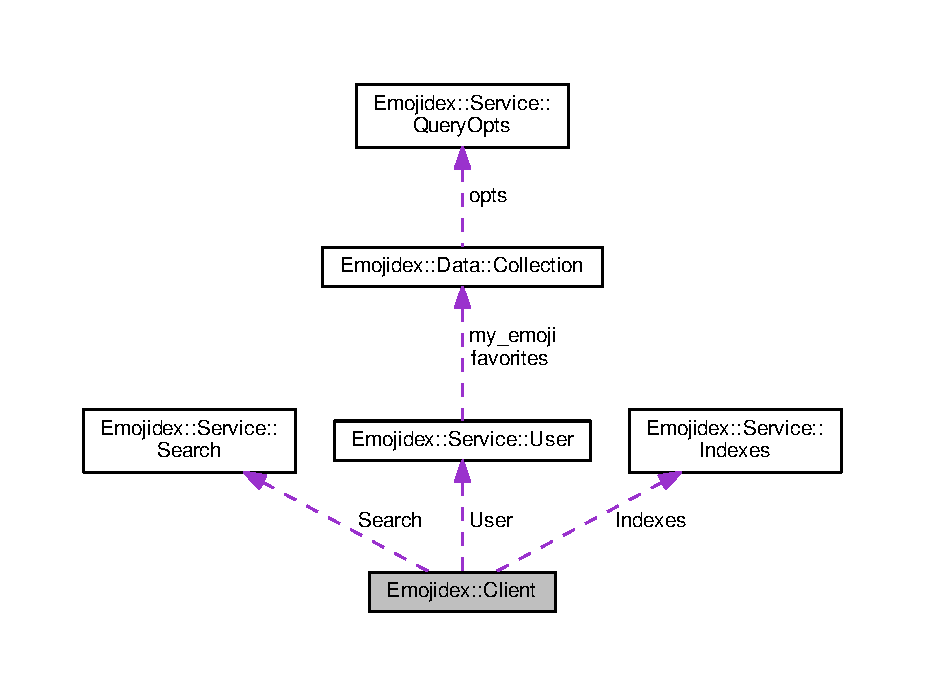
\includegraphics[width=350pt]{classEmojidex_1_1Client__coll__graph}
\end{center}
\end{figure}
\subsection*{Public Member Functions}
\begin{DoxyCompactItemize}
\item 
char {\bfseries api\+Version} ()\hypertarget{classEmojidex_1_1Client_ada04f1b9d696a792184798e9021c4d1c}{}\label{classEmojidex_1_1Client_ada04f1b9d696a792184798e9021c4d1c}

\end{DoxyCompactItemize}
\subsection*{Public Attributes}
\begin{DoxyCompactItemize}
\item 
\hyperlink{classEmojidex_1_1Service_1_1User}{Emojidex\+::\+Service\+::\+User} $\ast$ \hyperlink{classEmojidex_1_1Client_aa81c4d93a3c5f7c052ec51480940bcf9}{User}\hypertarget{classEmojidex_1_1Client_aa81c4d93a3c5f7c052ec51480940bcf9}{}\label{classEmojidex_1_1Client_aa81c4d93a3c5f7c052ec51480940bcf9}

\begin{DoxyCompactList}\small\item\em \hyperlink{classEmojidex_1_1Client}{Client} user instance. \end{DoxyCompactList}\item 
\hyperlink{classEmojidex_1_1Service_1_1Search}{Emojidex\+::\+Service\+::\+Search} $\ast$ \hyperlink{classEmojidex_1_1Client_a78ab88058c7ae2b4ca94912da4dde033}{Search}\hypertarget{classEmojidex_1_1Client_a78ab88058c7ae2b4ca94912da4dde033}{}\label{classEmojidex_1_1Client_a78ab88058c7ae2b4ca94912da4dde033}

\begin{DoxyCompactList}\small\item\em \hyperlink{classEmojidex_1_1Client}{Client} search instance. \end{DoxyCompactList}\item 
\hyperlink{classEmojidex_1_1Service_1_1Indexes}{Emojidex\+::\+Service\+::\+Indexes} $\ast$ \hyperlink{classEmojidex_1_1Client_a1b05ff602e2be8497d6def01c52d5a23}{Indexes}\hypertarget{classEmojidex_1_1Client_a1b05ff602e2be8497d6def01c52d5a23}{}\label{classEmojidex_1_1Client_a1b05ff602e2be8497d6def01c52d5a23}

\begin{DoxyCompactList}\small\item\em \hyperlink{classEmojidex_1_1Client}{Client} index instance. \end{DoxyCompactList}\end{DoxyCompactItemize}


\subsection{Detailed Description}
Core client class (includes all components in a central state-\/machine client) 

In general you\textquotesingle{}ll want to run everything through a client as long as you are implementing something with a single user. Multiple client instances could produce unpredicable behaviour and should be avoided. By loggin in with the User instance of this client class user details will automatically be set on appropriate queries. 

The documentation for this class was generated from the following file\+:\begin{DoxyCompactItemize}
\item 
client.\+h\end{DoxyCompactItemize}

\hypertarget{classEmojidex_1_1Data_1_1Collection}{}\section{Emojidex\+:\+:Data\+:\+:Collection Class Reference}
\label{classEmojidex_1_1Data_1_1Collection}\index{Emojidex\+::\+Data\+::\+Collection@{Emojidex\+::\+Data\+::\+Collection}}


A managed collection of emoji objects.  




{\ttfamily \#include $<$collection.\+h$>$}



Collaboration diagram for Emojidex\+:\+:Data\+:\+:Collection\+:\nopagebreak
\begin{figure}[H]
\begin{center}
\leavevmode
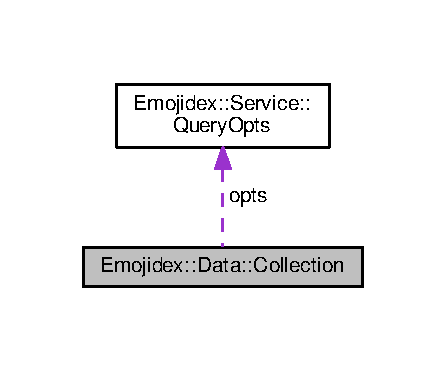
\includegraphics[width=214pt]{classEmojidex_1_1Data_1_1Collection__coll__graph}
\end{center}
\end{figure}
\subsection*{Public Member Functions}
\begin{DoxyCompactItemize}
\item 
std\+::vector$<$ \hyperlink{classEmojidex_1_1Data_1_1Emoji}{Emojidex\+::\+Data\+::\+Emoji} $>$ \hyperlink{classEmojidex_1_1Data_1_1Collection_a650a418293d89311263dc3e744416b1f}{all} ()\hypertarget{classEmojidex_1_1Data_1_1Collection_a650a418293d89311263dc3e744416b1f}{}\label{classEmojidex_1_1Data_1_1Collection_a650a418293d89311263dc3e744416b1f}

\begin{DoxyCompactList}\small\item\em Returns a vector array of all emoji in the collection. \end{DoxyCompactList}\item 
\hyperlink{classEmojidex_1_1Data_1_1Emoji}{Emojidex\+::\+Data\+::\+Emoji} \hyperlink{classEmojidex_1_1Data_1_1Collection_ab06d56b5d177f1e489d36c5ccf02b362}{add} (\hyperlink{classEmojidex_1_1Data_1_1Emoji}{Emojidex\+::\+Data\+::\+Emoji} new\+\_\+emoji)\hypertarget{classEmojidex_1_1Data_1_1Collection_ab06d56b5d177f1e489d36c5ccf02b362}{}\label{classEmojidex_1_1Data_1_1Collection_ab06d56b5d177f1e489d36c5ccf02b362}

\begin{DoxyCompactList}\small\item\em Adds an emoji to the map. \end{DoxyCompactList}\item 
bool \hyperlink{classEmojidex_1_1Data_1_1Collection_a1e149fc6e461293a80babfd7461b02f4}{remove} (std\+::string code)
\begin{DoxyCompactList}\small\item\em Removes an emoji from the map \mbox{[}by code\mbox{]}. \end{DoxyCompactList}\item 
\hyperlink{classEmojidex_1_1Data_1_1Emoji}{Emojidex\+::\+Data\+::\+Emoji} \hyperlink{classEmojidex_1_1Data_1_1Collection_a85b15d61175aee9cce9b42fe6c21cf80}{find\+By\+Moji} (std\+::string moji)\hypertarget{classEmojidex_1_1Data_1_1Collection_a85b15d61175aee9cce9b42fe6c21cf80}{}\label{classEmojidex_1_1Data_1_1Collection_a85b15d61175aee9cce9b42fe6c21cf80}

\begin{DoxyCompactList}\small\item\em Finds by moji\mbox{[}character\mbox{]}code (U\+TF emoji only) \end{DoxyCompactList}\item 
\hyperlink{classEmojidex_1_1Data_1_1Emoji}{Emojidex\+::\+Data\+::\+Emoji} \hyperlink{classEmojidex_1_1Data_1_1Collection_a5ba6be5a862e6e23b2a5c99e6d751615}{find\+By\+Code} (std\+::string code)\hypertarget{classEmojidex_1_1Data_1_1Collection_a5ba6be5a862e6e23b2a5c99e6d751615}{}\label{classEmojidex_1_1Data_1_1Collection_a5ba6be5a862e6e23b2a5c99e6d751615}

\begin{DoxyCompactList}\small\item\em Finds by emoji \mbox{[}short\mbox{]} code. \end{DoxyCompactList}\item 
\hyperlink{classEmojidex_1_1Data_1_1Emoji}{Emojidex\+::\+Data\+::\+Emoji} \hyperlink{classEmojidex_1_1Data_1_1Collection_a54f948efec77f14099defd7e6172a5b0}{find\+By\+Unicode} (std\+::string unicode)\hypertarget{classEmojidex_1_1Data_1_1Collection_a54f948efec77f14099defd7e6172a5b0}{}\label{classEmojidex_1_1Data_1_1Collection_a54f948efec77f14099defd7e6172a5b0}

\begin{DoxyCompactList}\small\item\em Finds by Unicode value (must be lower case) \end{DoxyCompactList}\item 
\hyperlink{classEmojidex_1_1Data_1_1Collection}{Emojidex\+::\+Data\+::\+Collection} \hyperlink{classEmojidex_1_1Data_1_1Collection_a230c9aae3e864b28cc25b94d861246bb}{category} (std\+::string category)\hypertarget{classEmojidex_1_1Data_1_1Collection_a230c9aae3e864b28cc25b94d861246bb}{}\label{classEmojidex_1_1Data_1_1Collection_a230c9aae3e864b28cc25b94d861246bb}

\begin{DoxyCompactList}\small\item\em Obtain a sub collection of emoji of the specified category. \end{DoxyCompactList}\item 
\hyperlink{classEmojidex_1_1Data_1_1Collection}{Emojidex\+::\+Data\+::\+Collection} $\ast$ \hyperlink{classEmojidex_1_1Data_1_1Collection_a8166fb4585d12aa2843e7625a4accff2}{merge} (\hyperlink{classEmojidex_1_1Data_1_1Collection}{Emojidex\+::\+Data\+::\+Collection} delta\+\_\+collection)
\begin{DoxyCompactList}\small\item\em Merge a collection with this collection. \end{DoxyCompactList}\item 
\hyperlink{classEmojidex_1_1Data_1_1Collection}{Emojidex\+::\+Data\+::\+Collection} $\ast$ {\bfseries operator$<$$<$} (\hyperlink{classEmojidex_1_1Data_1_1Collection}{Emojidex\+::\+Data\+::\+Collection} delta\+\_\+collection)\hypertarget{classEmojidex_1_1Data_1_1Collection_abe7026c359c5cd222d61d34f38b1ce5d}{}\label{classEmojidex_1_1Data_1_1Collection_abe7026c359c5cd222d61d34f38b1ce5d}

\item 
\hyperlink{classEmojidex_1_1Data_1_1Collection}{Emojidex\+::\+Data\+::\+Collection} $\ast$ \hyperlink{classEmojidex_1_1Data_1_1Collection_abc94265d1af0e39ab7b12bbae92d4e4b}{merge\+J\+S\+ON} (std\+::string json\+\_\+string)
\item 
\hyperlink{classEmojidex_1_1Data_1_1Collection}{Emojidex\+::\+Data\+::\+Collection} \hyperlink{classEmojidex_1_1Data_1_1Collection_a98118ea678e6b838e05f8d41f7ef7416}{more} ()
\begin{DoxyCompactList}\small\item\em Get more of the collection if the collection is paginated and has remaining pages. \end{DoxyCompactList}\item 
void \hyperlink{classEmojidex_1_1Data_1_1Collection_ad18c6580a9afb8c132d4c158337e1524}{set\+Pagination} (\hyperlink{classEmojidex_1_1Data_1_1Collection}{Collection}($\ast$more\+Method)(\hyperlink{classEmojidex_1_1Data_1_1Collection}{Emojidex\+::\+Data\+::\+Collection}), unsigned int starting\+\_\+page, unsigned int limit, bool detailed)\hypertarget{classEmojidex_1_1Data_1_1Collection_ad18c6580a9afb8c132d4c158337e1524}{}\label{classEmojidex_1_1Data_1_1Collection_ad18c6580a9afb8c132d4c158337e1524}

\begin{DoxyCompactList}\small\item\em Sets up collection as a paged collection (with more pages/emoji on the service). \end{DoxyCompactList}\end{DoxyCompactItemize}
\subsection*{Public Attributes}
\begin{DoxyCompactItemize}
\item 
std\+::unordered\+\_\+map$<$ std\+::string, \hyperlink{classEmojidex_1_1Data_1_1Emoji}{Emojidex\+::\+Data\+::\+Emoji} $>$ \hyperlink{classEmojidex_1_1Data_1_1Collection_aa8164e800401e64ce162ee5e734d9e74}{emoji}\hypertarget{classEmojidex_1_1Data_1_1Collection_aa8164e800401e64ce162ee5e734d9e74}{}\label{classEmojidex_1_1Data_1_1Collection_aa8164e800401e64ce162ee5e734d9e74}

\begin{DoxyCompactList}\small\item\em emoji data hash, mapped by code \end{DoxyCompactList}\item 
std\+::string \hyperlink{classEmojidex_1_1Data_1_1Collection_a937eedb36767877da7c793625bf919a6}{endpoint}\hypertarget{classEmojidex_1_1Data_1_1Collection_a937eedb36767877da7c793625bf919a6}{}\label{classEmojidex_1_1Data_1_1Collection_a937eedb36767877da7c793625bf919a6}

\begin{DoxyCompactList}\small\item\em The service endpoint this collection is derived from. \end{DoxyCompactList}\item 
\hyperlink{classEmojidex_1_1Service_1_1QueryOpts}{Emojidex\+::\+Service\+::\+Query\+Opts} \hyperlink{classEmojidex_1_1Data_1_1Collection_ade67a564b14f14375af66bc1a550ecdb}{opts}\hypertarget{classEmojidex_1_1Data_1_1Collection_ade67a564b14f14375af66bc1a550ecdb}{}\label{classEmojidex_1_1Data_1_1Collection_ade67a564b14f14375af66bc1a550ecdb}

\begin{DoxyCompactList}\small\item\em Query options on the endpoint. \end{DoxyCompactList}\item 
unsigned int \hyperlink{classEmojidex_1_1Data_1_1Collection_a0355662d1097dd631a6d6ce09875e8c3}{total\+\_\+count}\hypertarget{classEmojidex_1_1Data_1_1Collection_a0355662d1097dd631a6d6ce09875e8c3}{}\label{classEmojidex_1_1Data_1_1Collection_a0355662d1097dd631a6d6ce09875e8c3}

\begin{DoxyCompactList}\small\item\em The total number of emoji availble on the service to fill this collection. \end{DoxyCompactList}\end{DoxyCompactItemize}


\subsection{Detailed Description}
A managed collection of emoji objects. 

\subsection{Member Function Documentation}
\index{Emojidex\+::\+Data\+::\+Collection@{Emojidex\+::\+Data\+::\+Collection}!merge@{merge}}
\index{merge@{merge}!Emojidex\+::\+Data\+::\+Collection@{Emojidex\+::\+Data\+::\+Collection}}
\subsubsection[{\texorpdfstring{merge(\+Emojidex\+::\+Data\+::\+Collection delta\+\_\+collection)}{merge(Emojidex::Data::Collection delta_collection)}}]{\setlength{\rightskip}{0pt plus 5cm}{\bf Emojidex\+::\+Data\+::\+Collection}$\ast$ Emojidex\+::\+Data\+::\+Collection\+::merge (
\begin{DoxyParamCaption}
\item[{{\bf Emojidex\+::\+Data\+::\+Collection}}]{delta\+\_\+collection}
\end{DoxyParamCaption}
)}\hypertarget{classEmojidex_1_1Data_1_1Collection_a8166fb4585d12aa2843e7625a4accff2}{}\label{classEmojidex_1_1Data_1_1Collection_a8166fb4585d12aa2843e7625a4accff2}


Merge a collection with this collection. 

Overwrites emoji with the same code. Rerturns the joined collection after the merge for chaining. \index{Emojidex\+::\+Data\+::\+Collection@{Emojidex\+::\+Data\+::\+Collection}!merge\+J\+S\+ON@{merge\+J\+S\+ON}}
\index{merge\+J\+S\+ON@{merge\+J\+S\+ON}!Emojidex\+::\+Data\+::\+Collection@{Emojidex\+::\+Data\+::\+Collection}}
\subsubsection[{\texorpdfstring{merge\+J\+S\+O\+N(std\+::string json\+\_\+string)}{mergeJSON(std::string json_string)}}]{\setlength{\rightskip}{0pt plus 5cm}{\bf Emojidex\+::\+Data\+::\+Collection}$\ast$ Emojidex\+::\+Data\+::\+Collection\+::merge\+J\+S\+ON (
\begin{DoxyParamCaption}
\item[{std\+::string}]{json\+\_\+string}
\end{DoxyParamCaption}
)}\hypertarget{classEmojidex_1_1Data_1_1Collection_abc94265d1af0e39ab7b12bbae92d4e4b}{}\label{classEmojidex_1_1Data_1_1Collection_abc94265d1af0e39ab7b12bbae92d4e4b}
Add emoji from a J\+S\+ON string Returns this collection after the merge for chaining. \index{Emojidex\+::\+Data\+::\+Collection@{Emojidex\+::\+Data\+::\+Collection}!more@{more}}
\index{more@{more}!Emojidex\+::\+Data\+::\+Collection@{Emojidex\+::\+Data\+::\+Collection}}
\subsubsection[{\texorpdfstring{more()}{more()}}]{\setlength{\rightskip}{0pt plus 5cm}{\bf Emojidex\+::\+Data\+::\+Collection} Emojidex\+::\+Data\+::\+Collection\+::more (
\begin{DoxyParamCaption}
{}
\end{DoxyParamCaption}
)}\hypertarget{classEmojidex_1_1Data_1_1Collection_a98118ea678e6b838e05f8d41f7ef7416}{}\label{classEmojidex_1_1Data_1_1Collection_a98118ea678e6b838e05f8d41f7ef7416}


Get more of the collection if the collection is paginated and has remaining pages. 

Returns true if the next page was sucessfully obtained. Returns false if there are no more pages/emoji to obtain. \index{Emojidex\+::\+Data\+::\+Collection@{Emojidex\+::\+Data\+::\+Collection}!remove@{remove}}
\index{remove@{remove}!Emojidex\+::\+Data\+::\+Collection@{Emojidex\+::\+Data\+::\+Collection}}
\subsubsection[{\texorpdfstring{remove(std\+::string code)}{remove(std::string code)}}]{\setlength{\rightskip}{0pt plus 5cm}bool Emojidex\+::\+Data\+::\+Collection\+::remove (
\begin{DoxyParamCaption}
\item[{std\+::string}]{code}
\end{DoxyParamCaption}
)}\hypertarget{classEmojidex_1_1Data_1_1Collection_a1e149fc6e461293a80babfd7461b02f4}{}\label{classEmojidex_1_1Data_1_1Collection_a1e149fc6e461293a80babfd7461b02f4}


Removes an emoji from the map \mbox{[}by code\mbox{]}. 

Returns true if the emoji was located in the map and removed Returns false if the emoji was not located in the map 

The documentation for this class was generated from the following file\+:\begin{DoxyCompactItemize}
\item 
collection.\+h\end{DoxyCompactItemize}

\hypertarget{classEmojidex_1_1Service_1_1Collector}{}\section{Emojidex\+:\+:Service\+:\+:Collector Class Reference}
\label{classEmojidex_1_1Service_1_1Collector}\index{Emojidex\+::\+Service\+::\+Collector@{Emojidex\+::\+Service\+::\+Collector}}
\subsection*{Static Public Member Functions}
\begin{DoxyCompactItemize}
\item 
static \hyperlink{classEmojidex_1_1Data_1_1Collection}{Emojidex\+::\+Data\+::\+Collection} {\bfseries get\+Static\+Collection} (std\+::string name, std\+::string locale=D\+E\+F\+A\+U\+L\+T\+\_\+\+L\+O\+C\+A\+LE, bool detailed=true)\hypertarget{classEmojidex_1_1Service_1_1Collector_a51ed2454051cff8ee1b76dfe0ebd0e3c}{}\label{classEmojidex_1_1Service_1_1Collector_a51ed2454051cff8ee1b76dfe0ebd0e3c}

\item 
static \hyperlink{classEmojidex_1_1Data_1_1Collection}{Emojidex\+::\+Data\+::\+Collection} {\bfseries get\+Dynamic\+Collection} (std\+::string name, unsigned int page, unsigned int limit, bool detailed, \hyperlink{classEmojidex_1_1Service_1_1QueryOpts}{Emojidex\+::\+Service\+::\+Query\+Opts} $\ast$conditions=N\+U\+LL)\hypertarget{classEmojidex_1_1Service_1_1Collector_a3d576269475065aef15391dd597dfd5a}{}\label{classEmojidex_1_1Service_1_1Collector_a3d576269475065aef15391dd597dfd5a}

\item 
static \hyperlink{classEmojidex_1_1Data_1_1Collection}{Emojidex\+::\+Data\+::\+Collection} {\bfseries get\+Authorized\+Dynamic\+Collection} (std\+::string name, std\+::string auth\+\_\+token, unsigned int page, unsigned int limit, bool detailed, \hyperlink{classEmojidex_1_1Service_1_1QueryOpts}{Emojidex\+::\+Service\+::\+Query\+Opts} $\ast$conditions=N\+U\+LL)\hypertarget{classEmojidex_1_1Service_1_1Collector_a4d3839fcce3e4191b3076c64bab9a925}{}\label{classEmojidex_1_1Service_1_1Collector_a4d3839fcce3e4191b3076c64bab9a925}

\item 
static \hyperlink{classEmojidex_1_1Data_1_1Collection}{Emojidex\+::\+Data\+::\+Collection} {\bfseries get\+Collection} (\hyperlink{classEmojidex_1_1Data_1_1Collection}{Emojidex\+::\+Data\+::\+Collection} collect)\hypertarget{classEmojidex_1_1Service_1_1Collector_afeb2efb1c30de239a89f360eba795818}{}\label{classEmojidex_1_1Service_1_1Collector_afeb2efb1c30de239a89f360eba795818}

\end{DoxyCompactItemize}


The documentation for this class was generated from the following file\+:\begin{DoxyCompactItemize}
\item 
/home/zero/repo/emojidex/libemojidex/src/service/collector.\+h\end{DoxyCompactItemize}

\hypertarget{classEmojidex_1_1Data_1_1Emoji}{}\section{Emojidex\+:\+:Data\+:\+:Emoji Class Reference}
\label{classEmojidex_1_1Data_1_1Emoji}\index{Emojidex\+::\+Data\+::\+Emoji@{Emojidex\+::\+Data\+::\+Emoji}}


Collaboration diagram for Emojidex\+:\+:Data\+:\+:Emoji\+:\nopagebreak
\begin{figure}[H]
\begin{center}
\leavevmode
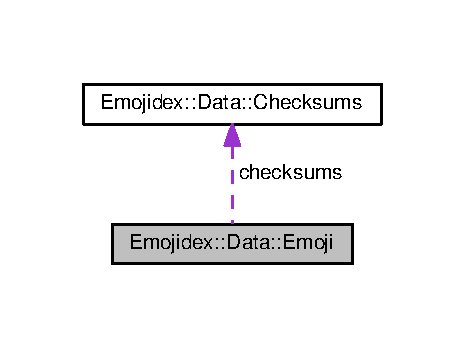
\includegraphics[width=223pt]{classEmojidex_1_1Data_1_1Emoji__coll__graph}
\end{center}
\end{figure}
\subsection*{Public Member Functions}
\begin{DoxyCompactItemize}
\item 
void {\bfseries fill\+From\+J\+S\+O\+N\+String} (std\+::string json)\hypertarget{classEmojidex_1_1Data_1_1Emoji_a81aa3a7621b4393bc211c4d67a153182}{}\label{classEmojidex_1_1Data_1_1Emoji_a81aa3a7621b4393bc211c4d67a153182}

\item 
void {\bfseries fill\+From\+J\+S\+ON} (rapidjson\+::\+Value \&d)\hypertarget{classEmojidex_1_1Data_1_1Emoji_ad173ee5dee8d6f6e807674fe7c73812f}{}\label{classEmojidex_1_1Data_1_1Emoji_ad173ee5dee8d6f6e807674fe7c73812f}

\end{DoxyCompactItemize}
\subsection*{Public Attributes}
\begin{DoxyCompactItemize}
\item 
std\+::string {\bfseries moji}\hypertarget{classEmojidex_1_1Data_1_1Emoji_a4503be17248d982d5574779ffc0bb2eb}{}\label{classEmojidex_1_1Data_1_1Emoji_a4503be17248d982d5574779ffc0bb2eb}

\item 
std\+::string {\bfseries code}\hypertarget{classEmojidex_1_1Data_1_1Emoji_ad098cea296b8389c4162467763effb72}{}\label{classEmojidex_1_1Data_1_1Emoji_ad098cea296b8389c4162467763effb72}

\item 
std\+::string {\bfseries unicode}\hypertarget{classEmojidex_1_1Data_1_1Emoji_a43e461b83bd1db8a8ca1f22b197a7a48}{}\label{classEmojidex_1_1Data_1_1Emoji_a43e461b83bd1db8a8ca1f22b197a7a48}

\item 
std\+::string {\bfseries category}\hypertarget{classEmojidex_1_1Data_1_1Emoji_a68441e044bc480a77e7fb0eaebd61d14}{}\label{classEmojidex_1_1Data_1_1Emoji_a68441e044bc480a77e7fb0eaebd61d14}

\item 
std\+::vector$<$ std\+::string $>$ {\bfseries tags}\hypertarget{classEmojidex_1_1Data_1_1Emoji_a31fc45978cc598ce1a22e8e9acb5ba44}{}\label{classEmojidex_1_1Data_1_1Emoji_a31fc45978cc598ce1a22e8e9acb5ba44}

\item 
std\+::string {\bfseries base}\hypertarget{classEmojidex_1_1Data_1_1Emoji_a91a8ecf38a8a36bda309ad290575c5e8}{}\label{classEmojidex_1_1Data_1_1Emoji_a91a8ecf38a8a36bda309ad290575c5e8}

\item 
std\+::vector$<$ std\+::string $>$ {\bfseries variants}\hypertarget{classEmojidex_1_1Data_1_1Emoji_aa8550f5cba404cae07523abf7eba3ea8}{}\label{classEmojidex_1_1Data_1_1Emoji_aa8550f5cba404cae07523abf7eba3ea8}

\item 
std\+::string {\bfseries link}\hypertarget{classEmojidex_1_1Data_1_1Emoji_a0744da3356a9ad54a21f3f303fbae93b}{}\label{classEmojidex_1_1Data_1_1Emoji_a0744da3356a9ad54a21f3f303fbae93b}

\item 
bool {\bfseries is\+\_\+wide}\hypertarget{classEmojidex_1_1Data_1_1Emoji_ae4151c475bae84ea410bfefd5ab2bd9d}{}\label{classEmojidex_1_1Data_1_1Emoji_ae4151c475bae84ea410bfefd5ab2bd9d}

\item 
bool {\bfseries copyright\+\_\+lock}\hypertarget{classEmojidex_1_1Data_1_1Emoji_a95e1ae753363bddf0d063550262c811d}{}\label{classEmojidex_1_1Data_1_1Emoji_a95e1ae753363bddf0d063550262c811d}

\item 
unsigned int {\bfseries times\+\_\+used}\hypertarget{classEmojidex_1_1Data_1_1Emoji_a12b0bac434266f28c90f4029cf345281}{}\label{classEmojidex_1_1Data_1_1Emoji_a12b0bac434266f28c90f4029cf345281}

\item 
unsigned int {\bfseries times\+\_\+favorited}\hypertarget{classEmojidex_1_1Data_1_1Emoji_ac069cd3bd86d55df3f95ff3e553c52ca}{}\label{classEmojidex_1_1Data_1_1Emoji_ac069cd3bd86d55df3f95ff3e553c52ca}

\item 
int {\bfseries score}\hypertarget{classEmojidex_1_1Data_1_1Emoji_ad8c90a6c15d02e99f29dac204f1e38d2}{}\label{classEmojidex_1_1Data_1_1Emoji_ad8c90a6c15d02e99f29dac204f1e38d2}

\item 
std\+::string {\bfseries attribution}\hypertarget{classEmojidex_1_1Data_1_1Emoji_a0670281a397e7bf106c0661d57fa8f0a}{}\label{classEmojidex_1_1Data_1_1Emoji_a0670281a397e7bf106c0661d57fa8f0a}

\item 
std\+::string {\bfseries user\+\_\+id}\hypertarget{classEmojidex_1_1Data_1_1Emoji_a279314b6aa4626e05b1bf2bc7acb75d1}{}\label{classEmojidex_1_1Data_1_1Emoji_a279314b6aa4626e05b1bf2bc7acb75d1}

\item 
double {\bfseries current\+\_\+price}\hypertarget{classEmojidex_1_1Data_1_1Emoji_a7828abfde9015bb688be4a93624f9dfe}{}\label{classEmojidex_1_1Data_1_1Emoji_a7828abfde9015bb688be4a93624f9dfe}

\item 
bool {\bfseries primary}\hypertarget{classEmojidex_1_1Data_1_1Emoji_afec2932bf98282f36d96c038fcf1ae13}{}\label{classEmojidex_1_1Data_1_1Emoji_afec2932bf98282f36d96c038fcf1ae13}

\item 
bool {\bfseries permalock}\hypertarget{classEmojidex_1_1Data_1_1Emoji_a74e1049056e4dd3aa8dd4b5c08fcae1e}{}\label{classEmojidex_1_1Data_1_1Emoji_a74e1049056e4dd3aa8dd4b5c08fcae1e}

\item 
std\+::string {\bfseries registered\+\_\+at}\hypertarget{classEmojidex_1_1Data_1_1Emoji_a1bea369e1adc382cd1dc7c5c65cced03}{}\label{classEmojidex_1_1Data_1_1Emoji_a1bea369e1adc382cd1dc7c5c65cced03}

\item 
std\+::string {\bfseries link\+\_\+expiration}\hypertarget{classEmojidex_1_1Data_1_1Emoji_abd597aeadcd7200b1699b61b70b0b183}{}\label{classEmojidex_1_1Data_1_1Emoji_abd597aeadcd7200b1699b61b70b0b183}

\item 
std\+::string {\bfseries lock\+\_\+expiration}\hypertarget{classEmojidex_1_1Data_1_1Emoji_ab89f5f4534ea2f04093a314304514786}{}\label{classEmojidex_1_1Data_1_1Emoji_ab89f5f4534ea2f04093a314304514786}

\item 
unsigned int {\bfseries times\+\_\+changed}\hypertarget{classEmojidex_1_1Data_1_1Emoji_a259f6b01221b548c048612b1c73cdf95}{}\label{classEmojidex_1_1Data_1_1Emoji_a259f6b01221b548c048612b1c73cdf95}

\item 
unsigned int {\bfseries favorited}\hypertarget{classEmojidex_1_1Data_1_1Emoji_ace2b4c0ce6c36f8b8562f2494aa4c306}{}\label{classEmojidex_1_1Data_1_1Emoji_ace2b4c0ce6c36f8b8562f2494aa4c306}

\item 
\hyperlink{classEmojidex_1_1Data_1_1Checksums}{Emojidex\+::\+Data\+::\+Checksums} {\bfseries checksums}\hypertarget{classEmojidex_1_1Data_1_1Emoji_aa0c2638f3d68e538a247e22ad70f6255}{}\label{classEmojidex_1_1Data_1_1Emoji_aa0c2638f3d68e538a247e22ad70f6255}

\end{DoxyCompactItemize}


The documentation for this class was generated from the following file\+:\begin{DoxyCompactItemize}
\item 
/home/zero/repo/emojidex/libemojidex/src/data/emoji.\+h\end{DoxyCompactItemize}

\hypertarget{classEmojidex_1_1Service_1_1HistoryItem}{}\section{Emojidex\+:\+:Service\+:\+:History\+Item Class Reference}
\label{classEmojidex_1_1Service_1_1HistoryItem}\index{Emojidex\+::\+Service\+::\+History\+Item@{Emojidex\+::\+Service\+::\+History\+Item}}
\subsection*{Public Member Functions}
\begin{DoxyCompactItemize}
\item 
{\bfseries History\+Item} (std\+::string emoji\+\_\+code, unsigned int times\+\_\+used, std\+::string last\+\_\+used)\hypertarget{classEmojidex_1_1Service_1_1HistoryItem_a83d81f8c40be75796eabea667e1d7400}{}\label{classEmojidex_1_1Service_1_1HistoryItem_a83d81f8c40be75796eabea667e1d7400}

\end{DoxyCompactItemize}
\subsection*{Public Attributes}
\begin{DoxyCompactItemize}
\item 
std\+::string {\bfseries emoji\+\_\+code}\hypertarget{classEmojidex_1_1Service_1_1HistoryItem_a98d6de7de108b4154cf4a47585af2489}{}\label{classEmojidex_1_1Service_1_1HistoryItem_a98d6de7de108b4154cf4a47585af2489}

\item 
unsigned int {\bfseries times\+\_\+used}\hypertarget{classEmojidex_1_1Service_1_1HistoryItem_a1cbf38f7c53d500fc9be47dfdeed167d}{}\label{classEmojidex_1_1Service_1_1HistoryItem_a1cbf38f7c53d500fc9be47dfdeed167d}

\item 
std\+::string {\bfseries last\+\_\+used}\hypertarget{classEmojidex_1_1Service_1_1HistoryItem_ac023cfba66fd6d1122d7d7b99009d441}{}\label{classEmojidex_1_1Service_1_1HistoryItem_ac023cfba66fd6d1122d7d7b99009d441}

\item 
boost\+::posix\+\_\+time\+::ptime {\bfseries last\+\_\+used\+\_\+posix}\hypertarget{classEmojidex_1_1Service_1_1HistoryItem_a30ffecf28921ab7593c889335789dfb1}{}\label{classEmojidex_1_1Service_1_1HistoryItem_a30ffecf28921ab7593c889335789dfb1}

\end{DoxyCompactItemize}


The documentation for this class was generated from the following file\+:\begin{DoxyCompactItemize}
\item 
history\+\_\+item.\+h\end{DoxyCompactItemize}

\hypertarget{classEmojidex_1_1Service_1_1Indexes}{}\section{Emojidex\+:\+:Service\+:\+:Indexes Class Reference}
\label{classEmojidex_1_1Service_1_1Indexes}\index{Emojidex\+::\+Service\+::\+Indexes@{Emojidex\+::\+Service\+::\+Indexes}}


Retrieves data from emojidex indexes.  




{\ttfamily \#include $<$indexes.\+h$>$}

\subsection*{Public Member Functions}
\begin{DoxyCompactItemize}
\item 
void {\bfseries set\+User} (const \hyperlink{classEmojidex_1_1Service_1_1User}{Emojidex\+::\+Service\+::\+User} $\ast$user)\hypertarget{classEmojidex_1_1Service_1_1Indexes_a94824b67e2e46b7bf46e1ec9f0040226}{}\label{classEmojidex_1_1Service_1_1Indexes_a94824b67e2e46b7bf46e1ec9f0040226}

\item 
\hyperlink{classEmojidex_1_1Data_1_1MojiCodes}{Emojidex\+::\+Data\+::\+Moji\+Codes} \hyperlink{classEmojidex_1_1Service_1_1Indexes_aad2b2a930b7665cc9a195cbaf302eb49}{moji\+Codes} (std\+::string locale=D\+E\+F\+A\+U\+L\+T\+\_\+\+L\+O\+C\+A\+LE)\hypertarget{classEmojidex_1_1Service_1_1Indexes_aad2b2a930b7665cc9a195cbaf302eb49}{}\label{classEmojidex_1_1Service_1_1Indexes_aad2b2a930b7665cc9a195cbaf302eb49}

\begin{DoxyCompactList}\small\item\em Get standard U\+TF emoji info in 3 compact forms. \end{DoxyCompactList}\item 
\hyperlink{classEmojidex_1_1Data_1_1Collection}{Emojidex\+::\+Data\+::\+Collection} \hyperlink{classEmojidex_1_1Service_1_1Indexes_a0c2b3e28fe19af86b556a9d5641ddeb4}{utf\+Emoji} (std\+::string locale=D\+E\+F\+A\+U\+L\+T\+\_\+\+L\+O\+C\+A\+LE, bool detailed=true)\hypertarget{classEmojidex_1_1Service_1_1Indexes_a0c2b3e28fe19af86b556a9d5641ddeb4}{}\label{classEmojidex_1_1Service_1_1Indexes_a0c2b3e28fe19af86b556a9d5641ddeb4}

\begin{DoxyCompactList}\small\item\em Get a collection of all standard U\+TF emoji. \end{DoxyCompactList}\item 
\hyperlink{classEmojidex_1_1Data_1_1Collection}{Emojidex\+::\+Data\+::\+Collection} \hyperlink{classEmojidex_1_1Service_1_1Indexes_a9106f50086dec7ff8496589883d5bd37}{extended\+Emoji} (std\+::string locale=D\+E\+F\+A\+U\+L\+T\+\_\+\+L\+O\+C\+A\+LE, bool detailed=true)\hypertarget{classEmojidex_1_1Service_1_1Indexes_a9106f50086dec7ff8496589883d5bd37}{}\label{classEmojidex_1_1Service_1_1Indexes_a9106f50086dec7ff8496589883d5bd37}

\begin{DoxyCompactList}\small\item\em Get a collection of all emojidex Extended emoji. \end{DoxyCompactList}\item 
\hyperlink{classEmojidex_1_1Data_1_1Collection}{Emojidex\+::\+Data\+::\+Collection} \hyperlink{classEmojidex_1_1Service_1_1Indexes_ac0aaddbd46779ced7502b6e1f4f81aa9}{emoji} (unsigned int page=D\+E\+F\+A\+U\+L\+T\+\_\+\+P\+A\+GE, unsigned int limit=D\+E\+F\+A\+U\+L\+T\+\_\+\+L\+I\+M\+IT, bool detailed=false, \hyperlink{classEmojidex_1_1Service_1_1QueryOpts}{Emojidex\+::\+Service\+::\+Query\+Opts} $\ast$conditions=N\+U\+LL)\hypertarget{classEmojidex_1_1Service_1_1Indexes_ac0aaddbd46779ced7502b6e1f4f81aa9}{}\label{classEmojidex_1_1Service_1_1Indexes_ac0aaddbd46779ced7502b6e1f4f81aa9}

\begin{DoxyCompactList}\small\item\em Get full emoji index (by score unless otherwise configured with conditions) \end{DoxyCompactList}\item 
\hyperlink{classEmojidex_1_1Data_1_1Collection}{Emojidex\+::\+Data\+::\+Collection} \hyperlink{classEmojidex_1_1Service_1_1Indexes_ab222e1830304388b081413dd0f9bac40}{newest} (std\+::string auth\+\_\+token=\char`\"{}\char`\"{}, unsigned int page=D\+E\+F\+A\+U\+L\+T\+\_\+\+P\+A\+GE, unsigned int limit=D\+E\+F\+A\+U\+L\+T\+\_\+\+L\+I\+M\+IT, bool detailed=false)\hypertarget{classEmojidex_1_1Service_1_1Indexes_ab222e1830304388b081413dd0f9bac40}{}\label{classEmojidex_1_1Service_1_1Indexes_ab222e1830304388b081413dd0f9bac40}

\begin{DoxyCompactList}\small\item\em Get Newest emoji. \end{DoxyCompactList}\item 
\hyperlink{classEmojidex_1_1Data_1_1Collection}{Emojidex\+::\+Data\+::\+Collection} \hyperlink{classEmojidex_1_1Service_1_1Indexes_ae32c731be5ae83b49b428ed7bfd4b2ed}{popular} (std\+::string auth\+\_\+token=\char`\"{}\char`\"{}, unsigned int page=D\+E\+F\+A\+U\+L\+T\+\_\+\+P\+A\+GE, unsigned int limit=D\+E\+F\+A\+U\+L\+T\+\_\+\+L\+I\+M\+IT, bool detailed=false)\hypertarget{classEmojidex_1_1Service_1_1Indexes_ae32c731be5ae83b49b428ed7bfd4b2ed}{}\label{classEmojidex_1_1Service_1_1Indexes_ae32c731be5ae83b49b428ed7bfd4b2ed}

\begin{DoxyCompactList}\small\item\em Get most Popular emoji. \end{DoxyCompactList}\item 
\hyperlink{classEmojidex_1_1Data_1_1Collection}{Emojidex\+::\+Data\+::\+Collection} \hyperlink{classEmojidex_1_1Service_1_1Indexes_ac489e53250311163cea342581ee5730d}{user\+Emoji} (std\+::string username, unsigned int page=D\+E\+F\+A\+U\+L\+T\+\_\+\+P\+A\+GE, unsigned int limit=D\+E\+F\+A\+U\+L\+T\+\_\+\+L\+I\+M\+IT, bool detailed=false)\hypertarget{classEmojidex_1_1Service_1_1Indexes_ac489e53250311163cea342581ee5730d}{}\label{classEmojidex_1_1Service_1_1Indexes_ac489e53250311163cea342581ee5730d}

\begin{DoxyCompactList}\small\item\em Get the emoji registered by a specific user (by username) \end{DoxyCompactList}\end{DoxyCompactItemize}


\subsection{Detailed Description}
Retrieves data from emojidex indexes. 

The documentation for this class was generated from the following file\+:\begin{DoxyCompactItemize}
\item 
indexes.\+h\end{DoxyCompactItemize}

\hypertarget{classEmojidex_1_1Data_1_1MojiCodes}{}\section{Emojidex\+:\+:Data\+:\+:Moji\+Codes Class Reference}
\label{classEmojidex_1_1Data_1_1MojiCodes}\index{Emojidex\+::\+Data\+::\+Moji\+Codes@{Emojidex\+::\+Data\+::\+Moji\+Codes}}


Moji \mbox{[}character\mbox{]} code container with 3 types of moji code indexes.  




{\ttfamily \#include $<$moji\+\_\+codes.\+h$>$}

\subsection*{Public Attributes}
\begin{DoxyCompactItemize}
\item 
std\+::string \hyperlink{classEmojidex_1_1Data_1_1MojiCodes_a30264352b96dfd99ff288c1669a999cc}{locale} = \char`\"{}\char`\"{}\hypertarget{classEmojidex_1_1Data_1_1MojiCodes_a30264352b96dfd99ff288c1669a999cc}{}\label{classEmojidex_1_1Data_1_1MojiCodes_a30264352b96dfd99ff288c1669a999cc}

\begin{DoxyCompactList}\small\item\em The locale of the codes in this instance. \end{DoxyCompactList}\item 
std\+::string \hyperlink{classEmojidex_1_1Data_1_1MojiCodes_af3d498cd68c0dad96394096631a871ce}{moji\+\_\+string}
\begin{DoxyCompactList}\small\item\em A large string of just emoji, sorted compount longest first. \end{DoxyCompactList}\item 
std\+::vector$<$ std\+::string $>$ \hyperlink{classEmojidex_1_1Data_1_1MojiCodes_a0847d05256542ad50fa8f3b48bf76853}{moji\+\_\+array}\hypertarget{classEmojidex_1_1Data_1_1MojiCodes_a0847d05256542ad50fa8f3b48bf76853}{}\label{classEmojidex_1_1Data_1_1MojiCodes_a0847d05256542ad50fa8f3b48bf76853}

\begin{DoxyCompactList}\small\item\em An array with each item containing a single emoji, compount longest first. \end{DoxyCompactList}\item 
std\+::unordered\+\_\+map$<$ std\+::string, std\+::string $>$ \hyperlink{classEmojidex_1_1Data_1_1MojiCodes_adaa77850c0d3d456c268a15e0f92e3ec}{moji\+\_\+index}\hypertarget{classEmojidex_1_1Data_1_1MojiCodes_adaa77850c0d3d456c268a15e0f92e3ec}{}\label{classEmojidex_1_1Data_1_1MojiCodes_adaa77850c0d3d456c268a15e0f92e3ec}

\begin{DoxyCompactList}\small\item\em A hash/map of emoji and their short codes in the given locale. \end{DoxyCompactList}\end{DoxyCompactItemize}


\subsection{Detailed Description}
Moji \mbox{[}character\mbox{]} code container with 3 types of moji code indexes. 

\subsection{Member Data Documentation}
\index{Emojidex\+::\+Data\+::\+Moji\+Codes@{Emojidex\+::\+Data\+::\+Moji\+Codes}!moji\+\_\+string@{moji\+\_\+string}}
\index{moji\+\_\+string@{moji\+\_\+string}!Emojidex\+::\+Data\+::\+Moji\+Codes@{Emojidex\+::\+Data\+::\+Moji\+Codes}}
\subsubsection[{\texorpdfstring{moji\+\_\+string}{moji_string}}]{\setlength{\rightskip}{0pt plus 5cm}std\+::string Emojidex\+::\+Data\+::\+Moji\+Codes\+::moji\+\_\+string}\hypertarget{classEmojidex_1_1Data_1_1MojiCodes_af3d498cd68c0dad96394096631a871ce}{}\label{classEmojidex_1_1Data_1_1MojiCodes_af3d498cd68c0dad96394096631a871ce}


A large string of just emoji, sorted compount longest first. 

Use this for regex to detect emoji within text or to validate emoji / determine if a charater is an emoji. 

The documentation for this class was generated from the following file\+:\begin{DoxyCompactItemize}
\item 
moji\+\_\+codes.\+h\end{DoxyCompactItemize}

\hypertarget{classEmojidex_1_1Service_1_1QueryOpts}{}\section{Emojidex\+:\+:Service\+:\+:Query\+Opts Class Reference}
\label{classEmojidex_1_1Service_1_1QueryOpts}\index{Emojidex\+::\+Service\+::\+Query\+Opts@{Emojidex\+::\+Service\+::\+Query\+Opts}}
\subsection*{Public Member Functions}
\begin{DoxyCompactItemize}
\item 
void {\bfseries set\+Collection\+Defaults} ()\hypertarget{classEmojidex_1_1Service_1_1QueryOpts_a8644a708f05f9cc96d2a58021c2c58ad}{}\label{classEmojidex_1_1Service_1_1QueryOpts_a8644a708f05f9cc96d2a58021c2c58ad}

\item 
\hyperlink{classEmojidex_1_1Service_1_1QueryOpts}{Emojidex\+::\+Service\+::\+Query\+Opts} \& {\bfseries locale} (const std\+::string \&locale=D\+E\+F\+A\+U\+L\+T\+\_\+\+L\+O\+C\+A\+LE)\hypertarget{classEmojidex_1_1Service_1_1QueryOpts_aaf1f11b06b53a16a21a664225b16ddd6}{}\label{classEmojidex_1_1Service_1_1QueryOpts_aaf1f11b06b53a16a21a664225b16ddd6}

\item 
const std\+::string \& {\bfseries get\+Locale} () const \hypertarget{classEmojidex_1_1Service_1_1QueryOpts_a21ac7ce8f5aabc514b9febb5ef98c7a1}{}\label{classEmojidex_1_1Service_1_1QueryOpts_a21ac7ce8f5aabc514b9febb5ef98c7a1}

\item 
\hyperlink{classEmojidex_1_1Service_1_1QueryOpts}{Emojidex\+::\+Service\+::\+Query\+Opts} \& {\bfseries page} (unsigned int number=D\+E\+F\+A\+U\+L\+T\+\_\+\+P\+A\+GE)\hypertarget{classEmojidex_1_1Service_1_1QueryOpts_a09de9071d7d678fc2cbfd3b625261b22}{}\label{classEmojidex_1_1Service_1_1QueryOpts_a09de9071d7d678fc2cbfd3b625261b22}

\item 
unsigned int {\bfseries get\+Page} () const \hypertarget{classEmojidex_1_1Service_1_1QueryOpts_ab09d80f6810994e9f17eb69e0bf5bbd2}{}\label{classEmojidex_1_1Service_1_1QueryOpts_ab09d80f6810994e9f17eb69e0bf5bbd2}

\item 
\hyperlink{classEmojidex_1_1Service_1_1QueryOpts}{Emojidex\+::\+Service\+::\+Query\+Opts} \& {\bfseries limit} (unsigned int value=D\+E\+F\+A\+U\+L\+T\+\_\+\+L\+I\+M\+IT)\hypertarget{classEmojidex_1_1Service_1_1QueryOpts_a3a462f0647c4229aa24016c7e3fc24ea}{}\label{classEmojidex_1_1Service_1_1QueryOpts_a3a462f0647c4229aa24016c7e3fc24ea}

\item 
unsigned int {\bfseries get\+Limit} () const \hypertarget{classEmojidex_1_1Service_1_1QueryOpts_a1ad7569bc9fb0ab58ededdad2977e00f}{}\label{classEmojidex_1_1Service_1_1QueryOpts_a1ad7569bc9fb0ab58ededdad2977e00f}

\item 
\hyperlink{classEmojidex_1_1Service_1_1QueryOpts}{Emojidex\+::\+Service\+::\+Query\+Opts} \& {\bfseries detailed} (bool detail=true)\hypertarget{classEmojidex_1_1Service_1_1QueryOpts_a3cca92ff06d005a40e768ea9157721b6}{}\label{classEmojidex_1_1Service_1_1QueryOpts_a3cca92ff06d005a40e768ea9157721b6}

\item 
bool {\bfseries get\+Detailed} () const \hypertarget{classEmojidex_1_1Service_1_1QueryOpts_ae48076b7bd5daa429ebea6f767e5304f}{}\label{classEmojidex_1_1Service_1_1QueryOpts_ae48076b7bd5daa429ebea6f767e5304f}

\item 
\hyperlink{classEmojidex_1_1Service_1_1QueryOpts}{Emojidex\+::\+Service\+::\+Query\+Opts} \& {\bfseries username} (const std\+::string \&username=\char`\"{}\char`\"{})\hypertarget{classEmojidex_1_1Service_1_1QueryOpts_ae4216a7709c4ecda00f5f347662f8f65}{}\label{classEmojidex_1_1Service_1_1QueryOpts_ae4216a7709c4ecda00f5f347662f8f65}

\item 
const std\+::string \& {\bfseries get\+Username} () const \hypertarget{classEmojidex_1_1Service_1_1QueryOpts_ad36b0b5169a96133f3f55db3322bf754}{}\label{classEmojidex_1_1Service_1_1QueryOpts_ad36b0b5169a96133f3f55db3322bf754}

\item 
\hyperlink{classEmojidex_1_1Service_1_1QueryOpts}{Emojidex\+::\+Service\+::\+Query\+Opts} \& {\bfseries auth\+\_\+token} (const std\+::string \&auth\+\_\+token=\char`\"{}\char`\"{})\hypertarget{classEmojidex_1_1Service_1_1QueryOpts_acca0bdf9bffb60ac767cff0506bc0fcc}{}\label{classEmojidex_1_1Service_1_1QueryOpts_acca0bdf9bffb60ac767cff0506bc0fcc}

\item 
const std\+::string \& {\bfseries get\+Auth\+Token} () const \hypertarget{classEmojidex_1_1Service_1_1QueryOpts_a26f673a87e58f3576e507321cb879eb8}{}\label{classEmojidex_1_1Service_1_1QueryOpts_a26f673a87e58f3576e507321cb879eb8}

\item 
\hyperlink{classEmojidex_1_1Service_1_1QueryOpts}{Emojidex\+::\+Service\+::\+Query\+Opts} \& {\bfseries tag} (const std\+::string \&tag)\hypertarget{classEmojidex_1_1Service_1_1QueryOpts_ab0d2aa112c6ad9c9dadaec0e48b39f3d}{}\label{classEmojidex_1_1Service_1_1QueryOpts_ab0d2aa112c6ad9c9dadaec0e48b39f3d}

\item 
\hyperlink{classEmojidex_1_1Service_1_1QueryOpts}{Emojidex\+::\+Service\+::\+Query\+Opts} \& {\bfseries clear\+Tags} ()\hypertarget{classEmojidex_1_1Service_1_1QueryOpts_a04cb66831c992b892b1ca80228bcffae}{}\label{classEmojidex_1_1Service_1_1QueryOpts_a04cb66831c992b892b1ca80228bcffae}

\item 
const std\+::vector$<$ std\+::string $>$ \& {\bfseries get\+Tags} () const \hypertarget{classEmojidex_1_1Service_1_1QueryOpts_a0085f26b918a3466ea8524e754f30598}{}\label{classEmojidex_1_1Service_1_1QueryOpts_a0085f26b918a3466ea8524e754f30598}

\item 
\hyperlink{classEmojidex_1_1Service_1_1QueryOpts}{Emojidex\+::\+Service\+::\+Query\+Opts} \& {\bfseries category} (const std\+::string \&category)\hypertarget{classEmojidex_1_1Service_1_1QueryOpts_a55bf6248156ed527d0cb1a469488c999}{}\label{classEmojidex_1_1Service_1_1QueryOpts_a55bf6248156ed527d0cb1a469488c999}

\item 
\hyperlink{classEmojidex_1_1Service_1_1QueryOpts}{Emojidex\+::\+Service\+::\+Query\+Opts} \& {\bfseries clear\+Categories} ()\hypertarget{classEmojidex_1_1Service_1_1QueryOpts_ad319ea44268d12872d7440697f86477a}{}\label{classEmojidex_1_1Service_1_1QueryOpts_ad319ea44268d12872d7440697f86477a}

\item 
const std\+::vector$<$ std\+::string $>$ \& {\bfseries get\+Categories} () const \hypertarget{classEmojidex_1_1Service_1_1QueryOpts_a70793f0fdaf87d80eb5343c45a58367e}{}\label{classEmojidex_1_1Service_1_1QueryOpts_a70793f0fdaf87d80eb5343c45a58367e}

\item 
\hyperlink{classEmojidex_1_1Service_1_1QueryOpts}{Emojidex\+::\+Service\+::\+Query\+Opts} \& {\bfseries set\+Sort} (std\+::string order=\char`\"{}\char`\"{})\hypertarget{classEmojidex_1_1Service_1_1QueryOpts_a5a187d4a45d838387f99196a70458173}{}\label{classEmojidex_1_1Service_1_1QueryOpts_a5a187d4a45d838387f99196a70458173}

\item 
\hyperlink{classEmojidex_1_1Service_1_1QueryOpts}{Emojidex\+::\+Service\+::\+Query\+Opts} \& {\bfseries ext} (const std\+::string \&opt, const std\+::string \&prefix=\char`\"{}\&\char`\"{})\hypertarget{classEmojidex_1_1Service_1_1QueryOpts_abc3b57ad07108e262eda4505cfdcc5c8}{}\label{classEmojidex_1_1Service_1_1QueryOpts_abc3b57ad07108e262eda4505cfdcc5c8}

\item 
\hyperlink{classEmojidex_1_1Service_1_1QueryOpts}{Emojidex\+::\+Service\+::\+Query\+Opts} \& {\bfseries clear\+Ext} ()\hypertarget{classEmojidex_1_1Service_1_1QueryOpts_ae0455c295169a616efbbd5b3721c998f}{}\label{classEmojidex_1_1Service_1_1QueryOpts_ae0455c295169a616efbbd5b3721c998f}

\item 
const std\+::string \& {\bfseries get\+Ext} () const \hypertarget{classEmojidex_1_1Service_1_1QueryOpts_ae1904d52159992a8bc6b50eefe2f27c6}{}\label{classEmojidex_1_1Service_1_1QueryOpts_ae1904d52159992a8bc6b50eefe2f27c6}

\item 
\hyperlink{classEmojidex_1_1Service_1_1QueryOpts}{Emojidex\+::\+Service\+::\+Query\+Opts} \& {\bfseries parse\+Unordered\+Map} (const std\+::unordered\+\_\+map$<$ std\+::string, std\+::string $>$ \&source\+\_\+map)\hypertarget{classEmojidex_1_1Service_1_1QueryOpts_afeace74ce515ca48c21c01fae5c01838}{}\label{classEmojidex_1_1Service_1_1QueryOpts_afeace74ce515ca48c21c01fae5c01838}

\item 
std\+::string {\bfseries to\+\_\+string} () const \hypertarget{classEmojidex_1_1Service_1_1QueryOpts_a8a513409a7f1c5509bd393bb2bd28225}{}\label{classEmojidex_1_1Service_1_1QueryOpts_a8a513409a7f1c5509bd393bb2bd28225}

\end{DoxyCompactItemize}


The documentation for this class was generated from the following file\+:\begin{DoxyCompactItemize}
\item 
/home/zero/repo/emojidex/libemojidex/src/service/query\+\_\+opts.\+h\end{DoxyCompactItemize}

\hypertarget{classEmojidex_1_1Service_1_1Search}{}\section{Emojidex\+:\+:Service\+:\+:Search Class Reference}
\label{classEmojidex_1_1Service_1_1Search}\index{Emojidex\+::\+Service\+::\+Search@{Emojidex\+::\+Service\+::\+Search}}
\subsection*{Public Member Functions}
\begin{DoxyCompactItemize}
\item 
void {\bfseries set\+User} (const \hyperlink{classEmojidex_1_1Service_1_1User}{Emojidex\+::\+Service\+::\+User} $\ast$user)\hypertarget{classEmojidex_1_1Service_1_1Search_ac29e36bb5aed38c8443b4457691a3e7a}{}\label{classEmojidex_1_1Service_1_1Search_ac29e36bb5aed38c8443b4457691a3e7a}

\item 
\hyperlink{classEmojidex_1_1Data_1_1Collection}{Emojidex\+::\+Data\+::\+Collection} {\bfseries term} (const std\+::string code\+\_\+cont, \hyperlink{classEmojidex_1_1Service_1_1QueryOpts}{Emojidex\+::\+Service\+::\+Query\+Opts} $\ast$conditions=N\+U\+LL)\hypertarget{classEmojidex_1_1Service_1_1Search_a7e9de234cfa8cdfe52b9ad02778ec096}{}\label{classEmojidex_1_1Service_1_1Search_a7e9de234cfa8cdfe52b9ad02778ec096}

\item 
\hyperlink{classEmojidex_1_1Data_1_1Collection}{Emojidex\+::\+Data\+::\+Collection} {\bfseries starting} (std\+::string code\+\_\+sw, \hyperlink{classEmojidex_1_1Service_1_1QueryOpts}{Emojidex\+::\+Service\+::\+Query\+Opts} $\ast$conditions=N\+U\+LL)\hypertarget{classEmojidex_1_1Service_1_1Search_a7b90f2dab9c28d2dc971bb7494b4d291}{}\label{classEmojidex_1_1Service_1_1Search_a7b90f2dab9c28d2dc971bb7494b4d291}

\item 
\hyperlink{classEmojidex_1_1Data_1_1Collection}{Emojidex\+::\+Data\+::\+Collection} {\bfseries ending} (std\+::string code\+\_\+ew, \hyperlink{classEmojidex_1_1Service_1_1QueryOpts}{Emojidex\+::\+Service\+::\+Query\+Opts} $\ast$conditions=N\+U\+LL)\hypertarget{classEmojidex_1_1Service_1_1Search_a0c8100ad888ab404088cd44b07bc8b91}{}\label{classEmojidex_1_1Service_1_1Search_a0c8100ad888ab404088cd44b07bc8b91}

\item 
\hyperlink{classEmojidex_1_1Data_1_1Collection}{Emojidex\+::\+Data\+::\+Collection} {\bfseries tags} (const std\+::vector$<$ std\+::string $>$ \&tags, \hyperlink{classEmojidex_1_1Service_1_1QueryOpts}{Emojidex\+::\+Service\+::\+Query\+Opts} $\ast$conditions=N\+U\+LL)\hypertarget{classEmojidex_1_1Service_1_1Search_af8d1aaece57cd92bf8712493055f2ef6}{}\label{classEmojidex_1_1Service_1_1Search_af8d1aaece57cd92bf8712493055f2ef6}

\item 
\hyperlink{classEmojidex_1_1Data_1_1Collection}{Emojidex\+::\+Data\+::\+Collection} {\bfseries advanced} (std\+::string code\+\_\+cont, const std\+::vector$<$ std\+::string $>$ \&categories, const std\+::vector$<$ std\+::string $>$ \&tags, \hyperlink{classEmojidex_1_1Service_1_1QueryOpts}{Emojidex\+::\+Service\+::\+Query\+Opts} $\ast$conditions=N\+U\+LL)\hypertarget{classEmojidex_1_1Service_1_1Search_a2924585a8bb92c1b902477cabc154fb0}{}\label{classEmojidex_1_1Service_1_1Search_a2924585a8bb92c1b902477cabc154fb0}

\item 
\hyperlink{classEmojidex_1_1Data_1_1Emoji}{Emojidex\+::\+Data\+::\+Emoji} {\bfseries find} (std\+::string code, bool detailed=true)\hypertarget{classEmojidex_1_1Service_1_1Search_a80970b4a18e5bcc37a2a697de237e8aa}{}\label{classEmojidex_1_1Service_1_1Search_a80970b4a18e5bcc37a2a697de237e8aa}

\end{DoxyCompactItemize}
\subsection*{Public Attributes}
\begin{DoxyCompactItemize}
\item 
unsigned int {\bfseries current\+\_\+page}\hypertarget{classEmojidex_1_1Service_1_1Search_a8fe41d03f8c3013a021ad103c2ab4245}{}\label{classEmojidex_1_1Service_1_1Search_a8fe41d03f8c3013a021ad103c2ab4245}

\end{DoxyCompactItemize}


The documentation for this class was generated from the following file\+:\begin{DoxyCompactItemize}
\item 
search.\+h\end{DoxyCompactItemize}

\hypertarget{classEmojidex_1_1Service_1_1Settings}{}\section{Emojidex\+:\+:Service\+:\+:Settings Class Reference}
\label{classEmojidex_1_1Service_1_1Settings}\index{Emojidex\+::\+Service\+::\+Settings@{Emojidex\+::\+Service\+::\+Settings}}
\subsection*{Static Public Attributes}
\begin{DoxyCompactItemize}
\item 
static bool {\bfseries initialized}\hypertarget{classEmojidex_1_1Service_1_1Settings_af71baa4b94fd1dabfbcb0fef7e40e551}{}\label{classEmojidex_1_1Service_1_1Settings_af71baa4b94fd1dabfbcb0fef7e40e551}

\item 
static std\+::string {\bfseries api\+\_\+host}\hypertarget{classEmojidex_1_1Service_1_1Settings_a5192b05e10865349f7531e9b48f059d3}{}\label{classEmojidex_1_1Service_1_1Settings_a5192b05e10865349f7531e9b48f059d3}

\item 
static std\+::string {\bfseries api\+\_\+prefix}\hypertarget{classEmojidex_1_1Service_1_1Settings_a91475013a914fb4a5b557a7bb9fa84a6}{}\label{classEmojidex_1_1Service_1_1Settings_a91475013a914fb4a5b557a7bb9fa84a6}

\item 
static std\+::string {\bfseries api\+\_\+protocol}\hypertarget{classEmojidex_1_1Service_1_1Settings_a102c707a10874ba2db39222153d230ef}{}\label{classEmojidex_1_1Service_1_1Settings_a102c707a10874ba2db39222153d230ef}

\item 
static std\+::string {\bfseries cdn\+\_\+host}\hypertarget{classEmojidex_1_1Service_1_1Settings_aafcb2e6bd54ab9773a450282b7e76773}{}\label{classEmojidex_1_1Service_1_1Settings_aafcb2e6bd54ab9773a450282b7e76773}

\item 
static std\+::string {\bfseries cdn\+\_\+prefix}\hypertarget{classEmojidex_1_1Service_1_1Settings_a4540c869e1b27ee4bd9426ea7486c35e}{}\label{classEmojidex_1_1Service_1_1Settings_a4540c869e1b27ee4bd9426ea7486c35e}

\item 
static std\+::string {\bfseries cdn\+\_\+protocol}\hypertarget{classEmojidex_1_1Service_1_1Settings_a007200735113741cec8282054eda7338}{}\label{classEmojidex_1_1Service_1_1Settings_a007200735113741cec8282054eda7338}

\item 
static bool {\bfseries closed\+\_\+net}\hypertarget{classEmojidex_1_1Service_1_1Settings_a4794a14aa2dda9d5e238c4b4c289e77c}{}\label{classEmojidex_1_1Service_1_1Settings_a4794a14aa2dda9d5e238c4b4c289e77c}

\item 
static std\+::string {\bfseries token}\hypertarget{classEmojidex_1_1Service_1_1Settings_a1aa303c664a4b238dd72c92e9660f3c4}{}\label{classEmojidex_1_1Service_1_1Settings_a1aa303c664a4b238dd72c92e9660f3c4}

\end{DoxyCompactItemize}


The documentation for this class was generated from the following file\+:\begin{DoxyCompactItemize}
\item 
settings.\+h\end{DoxyCompactItemize}

\hypertarget{classEmojidex_1_1Service_1_1Transactor}{}\section{Emojidex\+:\+:Service\+:\+:Transactor Class Reference}
\label{classEmojidex_1_1Service_1_1Transactor}\index{Emojidex\+::\+Service\+::\+Transactor@{Emojidex\+::\+Service\+::\+Transactor}}
\subsection*{Public Member Functions}
\begin{DoxyCompactItemize}
\item 
std\+::unordered\+\_\+map$<$ std\+::string, std\+::string $>$ {\bfseries query\+Template} (bool defaults=true)\hypertarget{classEmojidex_1_1Service_1_1Transactor_acdd10d6f4321b7a221c4bfb0d8590ff2}{}\label{classEmojidex_1_1Service_1_1Transactor_acdd10d6f4321b7a221c4bfb0d8590ff2}

\item 
std\+::string {\bfseries G\+ET} (const std\+::string \&endpoint, const std\+::unordered\+\_\+map$<$ std\+::string, std\+::string $>$ \&query=\{\{\char`\"{}\char`\"{},\char`\"{}\char`\"{}\}\}, int $\ast$status=N\+U\+LL)\hypertarget{classEmojidex_1_1Service_1_1Transactor_ad7db57d801c905c92ea81d0ae8e565b7}{}\label{classEmojidex_1_1Service_1_1Transactor_ad7db57d801c905c92ea81d0ae8e565b7}

\item 
std\+::string {\bfseries G\+ET} (const std\+::string \&endpoint, \hyperlink{classEmojidex_1_1Service_1_1QueryOpts}{Emojidex\+::\+Service\+::\+Query\+Opts} query, int $\ast$status=N\+U\+LL)\hypertarget{classEmojidex_1_1Service_1_1Transactor_aa21e59443304d5e9612981f4d7df4e8c}{}\label{classEmojidex_1_1Service_1_1Transactor_aa21e59443304d5e9612981f4d7df4e8c}

\item 
std\+::string {\bfseries P\+O\+ST} (const std\+::string \&endpoint, const std\+::unordered\+\_\+map$<$ std\+::string, std\+::string $>$ \&query=\{\{\char`\"{}\char`\"{},\char`\"{}\char`\"{}\}\}, int $\ast$status=N\+U\+LL)\hypertarget{classEmojidex_1_1Service_1_1Transactor_a5335a34c16a0d16bb0196fda4754b611}{}\label{classEmojidex_1_1Service_1_1Transactor_a5335a34c16a0d16bb0196fda4754b611}

\item 
std\+::string {\bfseries D\+E\+L\+E\+TE} (const std\+::string \&endpoint, const std\+::unordered\+\_\+map$<$ std\+::string, std\+::string $>$ \&query=\{\{\char`\"{}\char`\"{},\char`\"{}\char`\"{}\}\}, int $\ast$status=N\+U\+LL)\hypertarget{classEmojidex_1_1Service_1_1Transactor_a9e9d1edc59867650851b99129b6dcc1d}{}\label{classEmojidex_1_1Service_1_1Transactor_a9e9d1edc59867650851b99129b6dcc1d}

\end{DoxyCompactItemize}


The documentation for this class was generated from the following file\+:\begin{DoxyCompactItemize}
\item 
/home/zero/repo/emojidex/libemojidex/src/service/transactor.\+h\end{DoxyCompactItemize}

\hypertarget{classEmojidex_1_1Service_1_1User}{}\section{Emojidex\+:\+:Service\+:\+:User Class Reference}
\label{classEmojidex_1_1Service_1_1User}\index{Emojidex\+::\+Service\+::\+User@{Emojidex\+::\+Service\+::\+User}}


\hyperlink{classEmojidex_1_1Service_1_1User}{User} login/management for the emojidex service.  




{\ttfamily \#include $<$user.\+h$>$}



Collaboration diagram for Emojidex\+:\+:Service\+:\+:User\+:\nopagebreak
\begin{figure}[H]
\begin{center}
\leavevmode
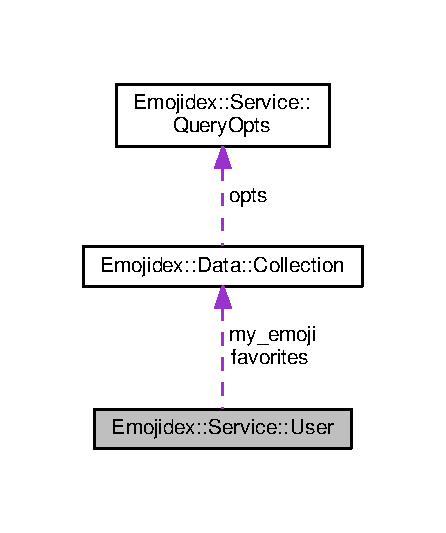
\includegraphics[width=214pt]{classEmojidex_1_1Service_1_1User__coll__graph}
\end{center}
\end{figure}
\subsection*{Public Types}
\begin{DoxyCompactItemize}
\item 
enum \hyperlink{classEmojidex_1_1Service_1_1User_a01490eed8fcfc954284a058fea0a242b}{Auth\+Status\+Code} \{ {\bfseries N\+O\+NE}, 
{\bfseries F\+A\+I\+L\+U\+RE}, 
{\bfseries U\+N\+V\+E\+R\+I\+F\+I\+ED}, 
{\bfseries V\+E\+R\+I\+F\+I\+ED}
 \}\hypertarget{classEmojidex_1_1Service_1_1User_a01490eed8fcfc954284a058fea0a242b}{}\label{classEmojidex_1_1Service_1_1User_a01490eed8fcfc954284a058fea0a242b}
\begin{DoxyCompactList}\small\item\em Status codes denoting the current authorization/login status of the user. \end{DoxyCompactList}
\end{DoxyCompactItemize}
\subsection*{Public Member Functions}
\begin{DoxyCompactItemize}
\item 
bool \hyperlink{classEmojidex_1_1Service_1_1User_a909f2f2858ed1978476fcc9e2f7b32c5}{authorize} (std\+::string \hyperlink{classEmojidex_1_1Service_1_1User_a5bb9d033735aa9f82fa666f811f48743}{username}, std\+::string token)\hypertarget{classEmojidex_1_1Service_1_1User_a909f2f2858ed1978476fcc9e2f7b32c5}{}\label{classEmojidex_1_1Service_1_1User_a909f2f2858ed1978476fcc9e2f7b32c5}

\begin{DoxyCompactList}\small\item\em Authroize the user with a username and auth\+\_\+token. \end{DoxyCompactList}\item 
bool \hyperlink{classEmojidex_1_1Service_1_1User_a44800534bd40a64caf35fc5fb93298c5}{login} (std\+::string user, std\+::string password)\hypertarget{classEmojidex_1_1Service_1_1User_a44800534bd40a64caf35fc5fb93298c5}{}\label{classEmojidex_1_1Service_1_1User_a44800534bd40a64caf35fc5fb93298c5}

\begin{DoxyCompactList}\small\item\em Authroize a user with a username or e-\/mail and password. \end{DoxyCompactList}\item 
bool \hyperlink{classEmojidex_1_1Service_1_1User_a4fd708d672d09325c07b72bae81bab10}{sync\+Favorites} (bool detailed=true)
\begin{DoxyCompactList}\small\item\em Synchronize user favorites from the emojidex service. \end{DoxyCompactList}\item 
bool \hyperlink{classEmojidex_1_1Service_1_1User_a69799b874e057eefccd36fdaae42695d}{add\+Favorite} (std\+::string code)\hypertarget{classEmojidex_1_1Service_1_1User_a69799b874e057eefccd36fdaae42695d}{}\label{classEmojidex_1_1Service_1_1User_a69799b874e057eefccd36fdaae42695d}

\begin{DoxyCompactList}\small\item\em Register an emoji to users favorites on the emojidex service. \end{DoxyCompactList}\item 
bool \hyperlink{classEmojidex_1_1Service_1_1User_a0f05215cbff6feacbe29ce9d7f1c2e17}{remove\+Favorite} (std\+::string code)\hypertarget{classEmojidex_1_1Service_1_1User_a0f05215cbff6feacbe29ce9d7f1c2e17}{}\label{classEmojidex_1_1Service_1_1User_a0f05215cbff6feacbe29ce9d7f1c2e17}

\begin{DoxyCompactList}\small\item\em Remove an emoji from users favorites on the emojidex service. \end{DoxyCompactList}\item 
std\+::vector$<$ \hyperlink{classEmojidex_1_1Service_1_1HistoryItem}{Emojidex\+::\+Service\+::\+History\+Item} $>$ \hyperlink{classEmojidex_1_1Service_1_1User_ae26cdfd2fbd24777a167709a615590d1}{sync\+History} (unsigned int page=0, unsigned int limit=D\+E\+F\+A\+U\+L\+T\+\_\+\+L\+I\+M\+IT)
\begin{DoxyCompactList}\small\item\em Syncronize history from the emojidex service. \end{DoxyCompactList}\item 
bool \hyperlink{classEmojidex_1_1Service_1_1User_a5bf74092c95f3b6aca6a5f8dee857879}{add\+History} (std\+::string code)\hypertarget{classEmojidex_1_1Service_1_1User_a5bf74092c95f3b6aca6a5f8dee857879}{}\label{classEmojidex_1_1Service_1_1User_a5bf74092c95f3b6aca6a5f8dee857879}

\begin{DoxyCompactList}\small\item\em Add an emoji to the users history. \end{DoxyCompactList}\item 
bool \hyperlink{classEmojidex_1_1Service_1_1User_acef94239cf65b7d8b707b688a8f0a4c9}{sync\+My\+Emoji} ()
\begin{DoxyCompactList}\small\item\em Sync users personal emoji. \end{DoxyCompactList}\item 
bool \hyperlink{classEmojidex_1_1Service_1_1User_a5d3d73e8788572961694cab846f5708a}{sync\+Following} ()\hypertarget{classEmojidex_1_1Service_1_1User_a5d3d73e8788572961694cab846f5708a}{}\label{classEmojidex_1_1Service_1_1User_a5d3d73e8788572961694cab846f5708a}

\begin{DoxyCompactList}\small\item\em Synchronizes the users following list. \end{DoxyCompactList}\item 
bool \hyperlink{classEmojidex_1_1Service_1_1User_ad0e6e27ef16bc37e1839d2deda9f8744}{add\+Following} (std\+::string \hyperlink{classEmojidex_1_1Service_1_1User_a5bb9d033735aa9f82fa666f811f48743}{username})\hypertarget{classEmojidex_1_1Service_1_1User_ad0e6e27ef16bc37e1839d2deda9f8744}{}\label{classEmojidex_1_1Service_1_1User_ad0e6e27ef16bc37e1839d2deda9f8744}

\begin{DoxyCompactList}\small\item\em Adds a user to the following list. \end{DoxyCompactList}\item 
bool \hyperlink{classEmojidex_1_1Service_1_1User_a42f548583cb236e22278754c863ea6c6}{remove\+Following} (std\+::string \hyperlink{classEmojidex_1_1Service_1_1User_a5bb9d033735aa9f82fa666f811f48743}{username})\hypertarget{classEmojidex_1_1Service_1_1User_a42f548583cb236e22278754c863ea6c6}{}\label{classEmojidex_1_1Service_1_1User_a42f548583cb236e22278754c863ea6c6}

\begin{DoxyCompactList}\small\item\em Removes a user from the following list. \end{DoxyCompactList}\item 
bool \hyperlink{classEmojidex_1_1Service_1_1User_ac9d62c8a7fd9eb6e64e930460e9f98d3}{sync\+Followers} ()\hypertarget{classEmojidex_1_1Service_1_1User_ac9d62c8a7fd9eb6e64e930460e9f98d3}{}\label{classEmojidex_1_1Service_1_1User_ac9d62c8a7fd9eb6e64e930460e9f98d3}

\begin{DoxyCompactList}\small\item\em Synchronizes followers from the emojidex service (Premium/\+Pro only) \end{DoxyCompactList}\end{DoxyCompactItemize}
\subsection*{Public Attributes}
\begin{DoxyCompactItemize}
\item 
\hyperlink{classEmojidex_1_1Service_1_1User_a01490eed8fcfc954284a058fea0a242b}{Auth\+Status\+Code} \hyperlink{classEmojidex_1_1Service_1_1User_adc84ddae4c153e0be58a904c97dd9096}{status}\hypertarget{classEmojidex_1_1Service_1_1User_adc84ddae4c153e0be58a904c97dd9096}{}\label{classEmojidex_1_1Service_1_1User_adc84ddae4c153e0be58a904c97dd9096}

\begin{DoxyCompactList}\small\item\em Holds the current status for this user instance (defaults to N\+O\+NE) \end{DoxyCompactList}\item 
std\+::string \hyperlink{classEmojidex_1_1Service_1_1User_a5bb9d033735aa9f82fa666f811f48743}{username}\hypertarget{classEmojidex_1_1Service_1_1User_a5bb9d033735aa9f82fa666f811f48743}{}\label{classEmojidex_1_1Service_1_1User_a5bb9d033735aa9f82fa666f811f48743}

\begin{DoxyCompactList}\small\item\em \hyperlink{classEmojidex_1_1Service_1_1User}{User} name of the user (defaults to \char`\"{}\char`\"{}) \end{DoxyCompactList}\item 
std\+::string \hyperlink{classEmojidex_1_1Service_1_1User_ab0dbc8fd015e529bdc295cbce221b6c3}{auth\+\_\+token}\hypertarget{classEmojidex_1_1Service_1_1User_ab0dbc8fd015e529bdc295cbce221b6c3}{}\label{classEmojidex_1_1Service_1_1User_ab0dbc8fd015e529bdc295cbce221b6c3}

\begin{DoxyCompactList}\small\item\em Authorization token of the user (defaults to \char`\"{}\char`\"{}) \end{DoxyCompactList}\item 
bool \hyperlink{classEmojidex_1_1Service_1_1User_a4e41f6c1d93b9c6cdf995904026ba761}{pro}\hypertarget{classEmojidex_1_1Service_1_1User_a4e41f6c1d93b9c6cdf995904026ba761}{}\label{classEmojidex_1_1Service_1_1User_a4e41f6c1d93b9c6cdf995904026ba761}

\begin{DoxyCompactList}\small\item\em True if the user has an active Pro account. \end{DoxyCompactList}\item 
std\+::string \hyperlink{classEmojidex_1_1Service_1_1User_a14d5753c674c9d6722d47982a309fc22}{pro\+\_\+exp}\hypertarget{classEmojidex_1_1Service_1_1User_a14d5753c674c9d6722d47982a309fc22}{}\label{classEmojidex_1_1Service_1_1User_a14d5753c674c9d6722d47982a309fc22}

\begin{DoxyCompactList}\small\item\em Ending date of Pro status (blank if user was never Pro) \end{DoxyCompactList}\item 
bool \hyperlink{classEmojidex_1_1Service_1_1User_a7ca897df6f9b7a903a395494b58a1b12}{premium}\hypertarget{classEmojidex_1_1Service_1_1User_a7ca897df6f9b7a903a395494b58a1b12}{}\label{classEmojidex_1_1Service_1_1User_a7ca897df6f9b7a903a395494b58a1b12}

\begin{DoxyCompactList}\small\item\em True if the user has an active Premium account. \end{DoxyCompactList}\item 
std\+::string \hyperlink{classEmojidex_1_1Service_1_1User_a310c157d017007a8747cb3fa03c29e78}{premium\+\_\+exp}\hypertarget{classEmojidex_1_1Service_1_1User_a310c157d017007a8747cb3fa03c29e78}{}\label{classEmojidex_1_1Service_1_1User_a310c157d017007a8747cb3fa03c29e78}

\begin{DoxyCompactList}\small\item\em Ending date of Premium status (blank if user was never Premium) \end{DoxyCompactList}\item 
bool \hyperlink{classEmojidex_1_1Service_1_1User_a0a66ff7c784815a1e186749bdc032070}{r18}\hypertarget{classEmojidex_1_1Service_1_1User_a0a66ff7c784815a1e186749bdc032070}{}\label{classEmojidex_1_1Service_1_1User_a0a66ff7c784815a1e186749bdc032070}

\begin{DoxyCompactList}\small\item\em True if the user has enabled viewing r18 \mbox{[}adult\mbox{]} content. \end{DoxyCompactList}\item 
\hyperlink{classEmojidex_1_1Data_1_1Collection}{Emojidex\+::\+Data\+::\+Collection} \hyperlink{classEmojidex_1_1Service_1_1User_a7f4e37b223204146363b50ffdf89e12e}{favorites}\hypertarget{classEmojidex_1_1Service_1_1User_a7f4e37b223204146363b50ffdf89e12e}{}\label{classEmojidex_1_1Service_1_1User_a7f4e37b223204146363b50ffdf89e12e}

\begin{DoxyCompactList}\small\item\em A collection of the emoji the user has favorited. \end{DoxyCompactList}\item 
std\+::vector$<$ \hyperlink{classEmojidex_1_1Service_1_1HistoryItem}{Emojidex\+::\+Service\+::\+History\+Item} $>$ \hyperlink{classEmojidex_1_1Service_1_1User_af3cc2fec42e5e17f442f718e15f76847}{history}\hypertarget{classEmojidex_1_1Service_1_1User_af3cc2fec42e5e17f442f718e15f76847}{}\label{classEmojidex_1_1Service_1_1User_af3cc2fec42e5e17f442f718e15f76847}

\begin{DoxyCompactList}\small\item\em An ordered vector of items in the users history. \end{DoxyCompactList}\item 
unsigned int \hyperlink{classEmojidex_1_1Service_1_1User_a5a7b4e141fdf8a9aaddfcce3394b12db}{history\+\_\+total}\hypertarget{classEmojidex_1_1Service_1_1User_a5a7b4e141fdf8a9aaddfcce3394b12db}{}\label{classEmojidex_1_1Service_1_1User_a5a7b4e141fdf8a9aaddfcce3394b12db}

\begin{DoxyCompactList}\small\item\em Total number of history items stored on the emojidex service. \end{DoxyCompactList}\item 
unsigned int \hyperlink{classEmojidex_1_1Service_1_1User_ab938b61c56121dbf590aa08d96556cd0}{history\+\_\+page}\hypertarget{classEmojidex_1_1Service_1_1User_ab938b61c56121dbf590aa08d96556cd0}{}\label{classEmojidex_1_1Service_1_1User_ab938b61c56121dbf590aa08d96556cd0}

\begin{DoxyCompactList}\small\item\em Current page of history items taken from the emojidex service. \end{DoxyCompactList}\item 
\hyperlink{classEmojidex_1_1Data_1_1Collection}{Emojidex\+::\+Data\+::\+Collection} \hyperlink{classEmojidex_1_1Service_1_1User_aa4b1decc97e13a92ba6830ccf2176f09}{my\+\_\+emoji}\hypertarget{classEmojidex_1_1Service_1_1User_aa4b1decc97e13a92ba6830ccf2176f09}{}\label{classEmojidex_1_1Service_1_1User_aa4b1decc97e13a92ba6830ccf2176f09}

\begin{DoxyCompactList}\small\item\em Collection of emoji the user has registered themselves. \end{DoxyCompactList}\item 
std\+::vector$<$ std\+::string $>$ \hyperlink{classEmojidex_1_1Service_1_1User_a48fb02c42de30f7b901f41fd74117839}{following}\hypertarget{classEmojidex_1_1Service_1_1User_a48fb02c42de30f7b901f41fd74117839}{}\label{classEmojidex_1_1Service_1_1User_a48fb02c42de30f7b901f41fd74117839}

\begin{DoxyCompactList}\small\item\em List of users the user is following. \end{DoxyCompactList}\item 
std\+::vector$<$ std\+::string $>$ \hyperlink{classEmojidex_1_1Service_1_1User_a89bd503730e389734980d45c978c6612}{followers}\hypertarget{classEmojidex_1_1Service_1_1User_a89bd503730e389734980d45c978c6612}{}\label{classEmojidex_1_1Service_1_1User_a89bd503730e389734980d45c978c6612}

\begin{DoxyCompactList}\small\item\em List of people following this user (Premium/\+Pro only) \end{DoxyCompactList}\end{DoxyCompactItemize}


\subsection{Detailed Description}
\hyperlink{classEmojidex_1_1Service_1_1User}{User} login/management for the emojidex service. 

\subsection{Member Function Documentation}
\index{Emojidex\+::\+Service\+::\+User@{Emojidex\+::\+Service\+::\+User}!sync\+Favorites@{sync\+Favorites}}
\index{sync\+Favorites@{sync\+Favorites}!Emojidex\+::\+Service\+::\+User@{Emojidex\+::\+Service\+::\+User}}
\subsubsection[{\texorpdfstring{sync\+Favorites(bool detailed=true)}{syncFavorites(bool detailed=true)}}]{\setlength{\rightskip}{0pt plus 5cm}bool Emojidex\+::\+Service\+::\+User\+::sync\+Favorites (
\begin{DoxyParamCaption}
\item[{bool}]{detailed = {\ttfamily true}}
\end{DoxyParamCaption}
)}\hypertarget{classEmojidex_1_1Service_1_1User_a4fd708d672d09325c07b72bae81bab10}{}\label{classEmojidex_1_1Service_1_1User_a4fd708d672d09325c07b72bae81bab10}


Synchronize user favorites from the emojidex service. 

Synchronizing clears the favorites collection and obtains the first page of favorites. Call favorites.\+more() to retreive consecutive pages. \index{Emojidex\+::\+Service\+::\+User@{Emojidex\+::\+Service\+::\+User}!sync\+History@{sync\+History}}
\index{sync\+History@{sync\+History}!Emojidex\+::\+Service\+::\+User@{Emojidex\+::\+Service\+::\+User}}
\subsubsection[{\texorpdfstring{sync\+History(unsigned int page=0, unsigned int limit=\+D\+E\+F\+A\+U\+L\+T\+\_\+\+L\+I\+M\+I\+T)}{syncHistory(unsigned int page=0, unsigned int limit=DEFAULT_LIMIT)}}]{\setlength{\rightskip}{0pt plus 5cm}std\+::vector$<${\bf Emojidex\+::\+Service\+::\+History\+Item}$>$ Emojidex\+::\+Service\+::\+User\+::sync\+History (
\begin{DoxyParamCaption}
\item[{unsigned int}]{page = {\ttfamily 0}, }
\item[{unsigned int}]{limit = {\ttfamily DEFAULT\+\_\+LIMIT}}
\end{DoxyParamCaption}
)}\hypertarget{classEmojidex_1_1Service_1_1User_ae26cdfd2fbd24777a167709a615590d1}{}\label{classEmojidex_1_1Service_1_1User_ae26cdfd2fbd24777a167709a615590d1}


Syncronize history from the emojidex service. 

Consecutive calls \mbox{[}with page set to 0\mbox{]} will get the next page after history\+\_\+page. The last page of history obtained is returned. \index{Emojidex\+::\+Service\+::\+User@{Emojidex\+::\+Service\+::\+User}!sync\+My\+Emoji@{sync\+My\+Emoji}}
\index{sync\+My\+Emoji@{sync\+My\+Emoji}!Emojidex\+::\+Service\+::\+User@{Emojidex\+::\+Service\+::\+User}}
\subsubsection[{\texorpdfstring{sync\+My\+Emoji()}{syncMyEmoji()}}]{\setlength{\rightskip}{0pt plus 5cm}bool Emojidex\+::\+Service\+::\+User\+::sync\+My\+Emoji (
\begin{DoxyParamCaption}
{}
\end{DoxyParamCaption}
)}\hypertarget{classEmojidex_1_1Service_1_1User_acef94239cf65b7d8b707b688a8f0a4c9}{}\label{classEmojidex_1_1Service_1_1User_acef94239cf65b7d8b707b688a8f0a4c9}


Sync users personal emoji. 

Synchronizing clears the my\+\_\+emoji collection. After sycronizing call my\+\_\+collection.\+more() to obtain consecutive pages of user emoji. 

The documentation for this class was generated from the following file\+:\begin{DoxyCompactItemize}
\item 
/home/zero/repo/emojidex/libemojidex/src/service/user.\+h\end{DoxyCompactItemize}

%--- End generated contents ---

% Index
\backmatter
\newpage
\phantomsection
\clearemptydoublepage
\addcontentsline{toc}{chapter}{Index}
\printindex

\end{document}
